\documentclass[11pt]{article}
\usepackage[T1]{fontenc}
\usepackage[margin=1in]{geometry}
\usepackage{amsmath,amssymb,amsthm,mathtools}
\usepackage{graphicx}
\usepackage{microtype}
\usepackage{xcolor}
\usepackage[colorlinks=true,linkcolor=blue!55!black,urlcolor=blue!65!black]{hyperref}

\newtheorem{theorem}{Theorem}
\newtheorem{corollary}[theorem]{Corollary}
\newtheorem{proposition}[theorem]{Proposition}
\newcommand{\Hh}{\mathcal H}

\title{No infinite-dimensional Hilbert space admits\\
a norm-compact exhaustion}
\author{Candidate full negative answer to the compact-exhaustion proposal\\
in arXiv:2512.24348}
\date{11 August 2026}

\begin{document}
\maketitle

\begin{center}
\fbox{\begin{minipage}{0.91\textwidth}
\textbf{Status: candidate counterexample/full classification, likely valid.}
With the standard norm topology, a Hilbert space admits a manifold-style
compact exhaustion if and only if it is finite-dimensional.  In particular,
the compact-exhaustion construction proposed for a nonseparable Hilbert space
cannot even be initiated.  This does not rule out heat kernels obtained by a
different approximation scheme or topology.
\end{minipage}}
\end{center}

\section{The source proposal}

Jorgensen, Jorgenson, and Smajlovic construct heat kernels on several
function spaces from parametrices.  In their final open-questions section
they recall the classical construction on a noncompact Riemannian manifold:
choose open sets $\Omega_j$ with compact closures satisfying
\[
  \overline{\Omega_j}\subset \Omega_{j+1},
  \qquad \bigcup_{j\ge 1}\Omega_j=M,
\]
and pass to a limit of the heat kernels on $\Omega_j$.  They then hypothesize
that a heat kernel on a nonseparable Hilbert space can similarly be defined
through compact exhaustion (arXiv:2512.24348v1, \S10.3, p.~34).  The complete source
page is reproduced next.

The natural topology on a Hilbert space in this analogy is its norm topology.
The obstruction below is purely topological and occurs before any analytic
choice of Laplacian, boundary condition, or convergence mode.

\clearpage
\begin{center}
  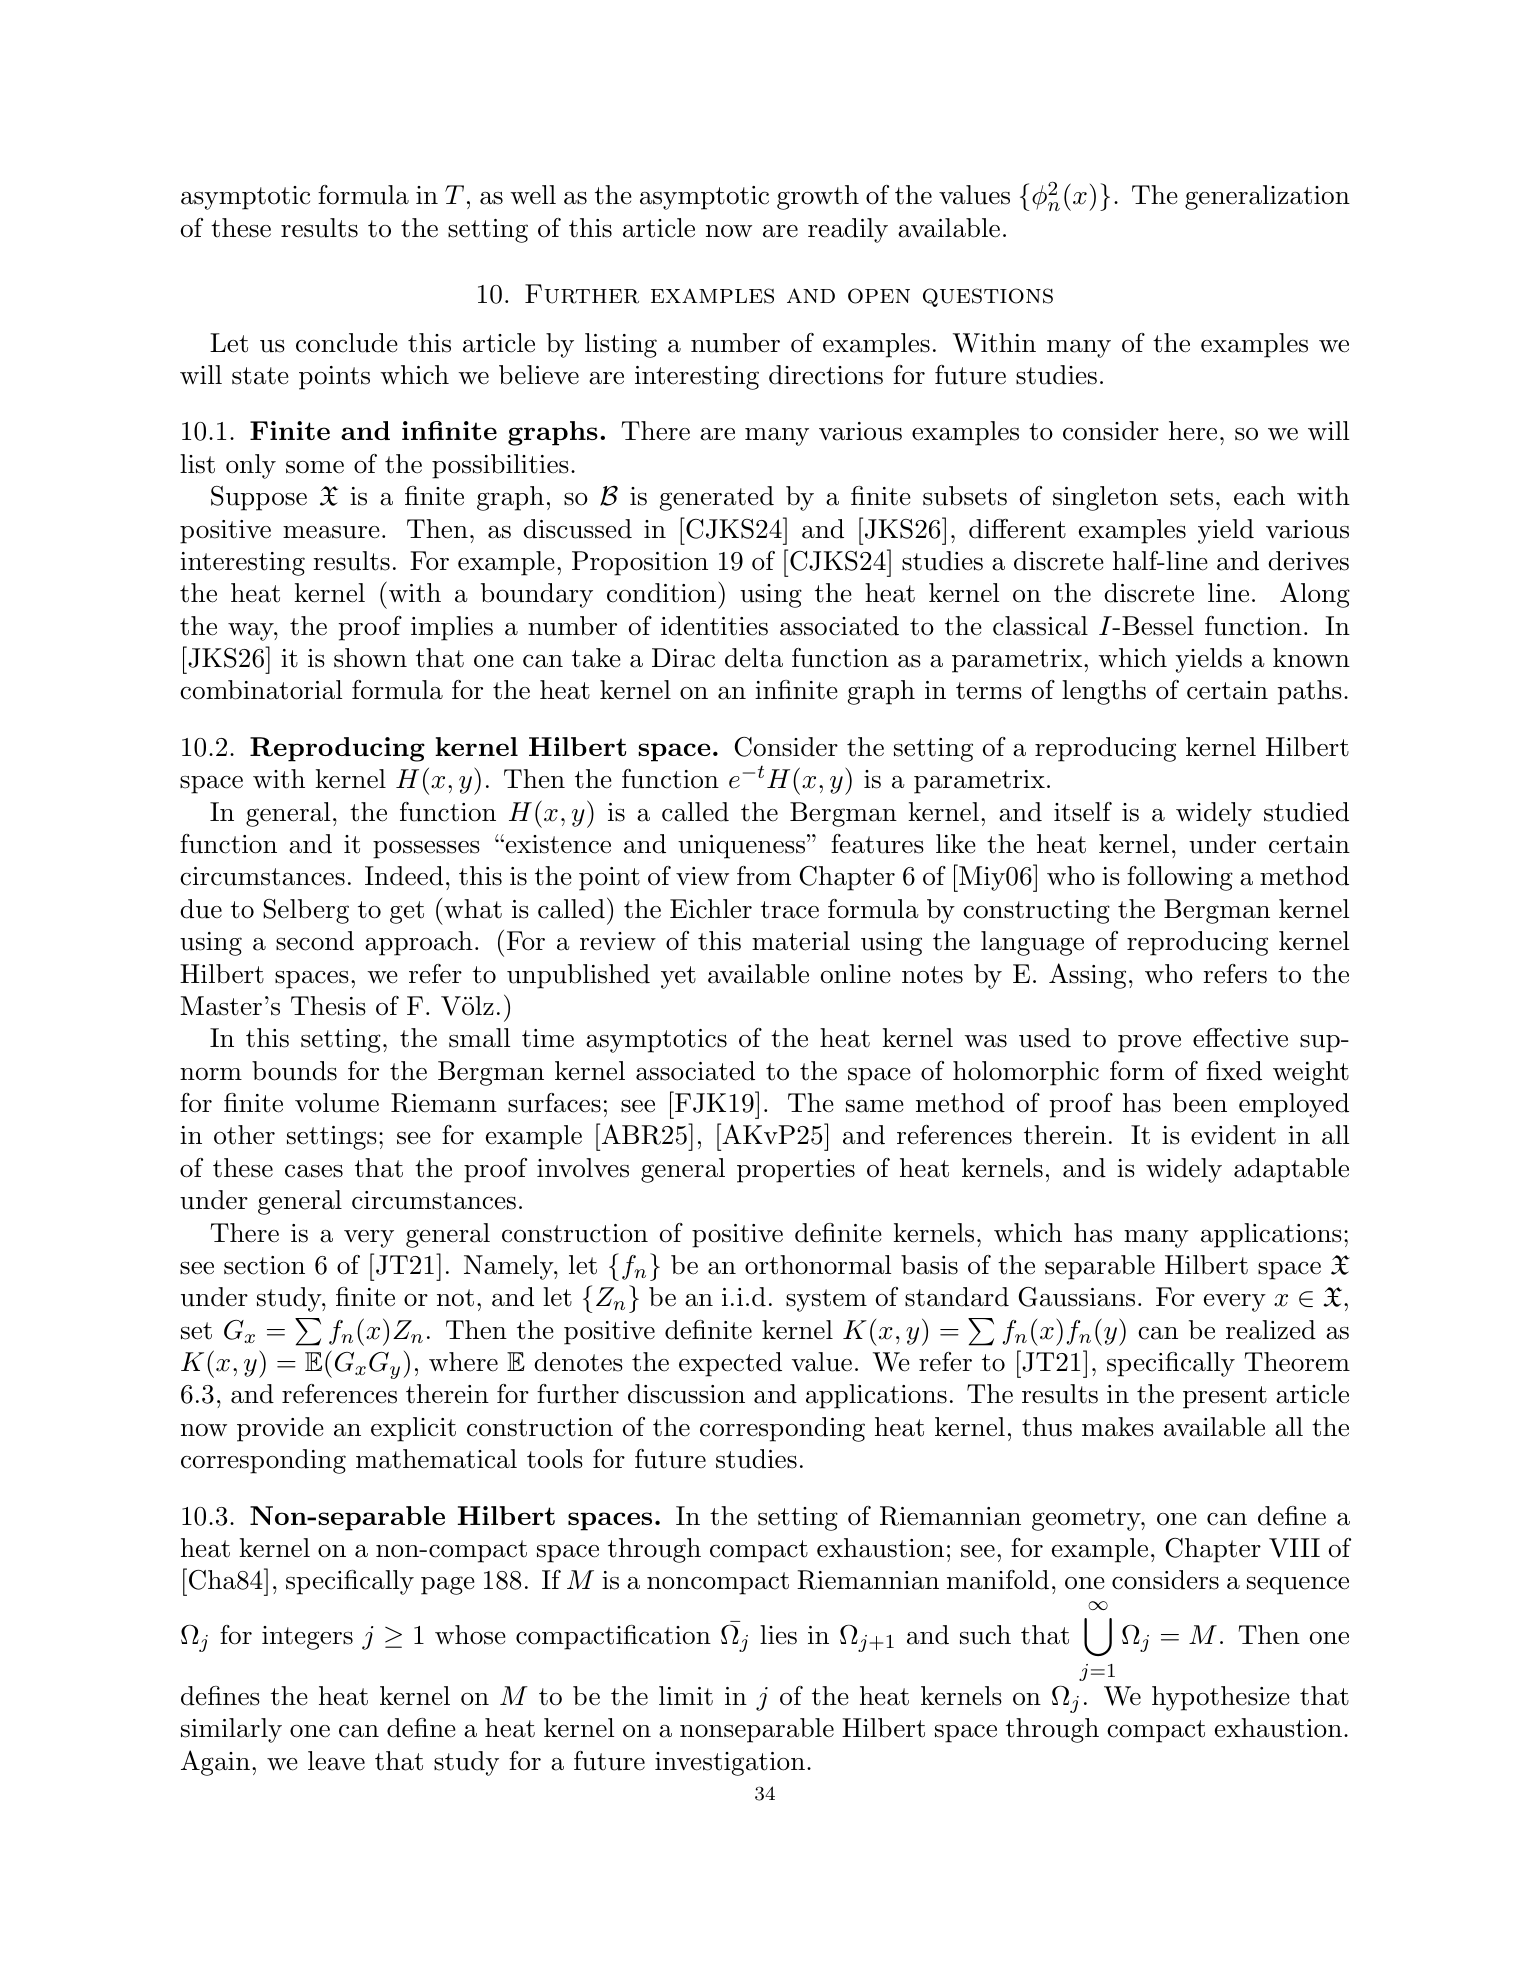
\includegraphics[width=\textwidth,height=0.92\textheight,keepaspectratio]
    {figures/source_open-34.png}
\end{center}

\clearpage
\section{Exact classification}

Call a sequence $(\Omega_j)_{j\ge1}$ a \emph{norm-compact exhaustion} of a
Hilbert space $\Hh$ if every $\Omega_j$ is norm open,
$\overline{\Omega_j}$ is norm compact,
$\overline{\Omega_j}\subset\Omega_{j+1}$, and
$\bigcup_j\Omega_j=\Hh$.  The nesting is not needed for the negative result.

\begin{theorem}\label{thm:classification}
For a real or complex Hilbert space $\Hh$, the following are equivalent.
\begin{enumerate}
  \item $\Hh$ admits a norm-compact exhaustion.
  \item $\Hh$ is a countable union of norm-compact subsets.
  \item $\Hh$ is finite-dimensional.
\end{enumerate}
\end{theorem}

\begin{proof}
The first condition implies the second because
$\Hh=\bigcup_j\overline{\Omega_j}$.

Suppose $\Hh=\bigcup_{j\ge1}K_j$ with each $K_j$ norm compact.  If $\Hh$ is
infinite-dimensional, every $K_j$ has empty interior.  Indeed, if
$B(x,r)\subset K_j$ for some $r>0$, then compactness and closedness give
$\overline B(x,r)\subset K_j$.  Translation by $-x$ and dilation by $1/r$
would make the closed unit ball of $\Hh$ compact.  This is impossible in an
infinite-dimensional normed space: Riesz's lemma supplies a sequence of unit
vectors with pairwise distance bounded below, hence with no convergent
subsequence.  Thus each compact $K_j$ is closed and nowhere dense.

But a Hilbert space is complete, so the Baire category theorem says that it
cannot be a countable union of closed nowhere-dense sets.  Hence $\Hh$ must
be finite-dimensional.

Conversely, if $\dim\Hh<\infty$, let $\Omega_j=B(0,j)$.  Heine--Borel gives
compactness of $\overline B(0,j)$, and
$\overline B(0,j)\subset B(0,j+1)$ gives the required strict nesting.
\end{proof}

\begin{corollary}\label{cor:source}
No nonseparable Hilbert space has the norm-compact exhaustion required by the
proposal in arXiv:2512.24348.  More strongly, no infinite-dimensional Hilbert
space has one, separable or not.
\end{corollary}

There is also a shorter obstruction tailored to the stated nonseparable
case.  Every compact metric space is separable, and a countable union of
separable subspaces is separable.  Therefore a nonseparable metric space can
never be $\sigma$-compact.  This argument needs neither linear structure nor
completeness; Theorem~\ref{thm:classification} gives the sharper
finite-dimensional classification.

\section{Why the manifold analogy breaks}

The Riemannian construction uses local compactness.  Every point lies in a
relatively compact coordinate neighborhood, and second countability lets
one select a countable exhaustion.  By contrast, a normed space is locally
compact exactly when it is finite-dimensional.  The proof above is the
global Baire-category form of the same obstruction.

Consequently, there are no norm-open domains $\Omega_j$ with compact norm
closures that cover an infinite-dimensional Hilbert space.  In particular,
there are no domain heat kernels of the proposed kind whose limit in $j$
could define the desired kernel.  The conjectured procedure fails at its
first geometric input, independently of every heat-kernel estimate.

\section{Deep upgrades and alternative readings}

\paragraph{Sequential separable approximations.}
The nonseparable obstruction persists after relaxing ``compact'' to
``separable.''  If $(S_j)$ is any sequence of separable subsets of a metric
space, then $\overline{\bigcup_jS_j}$ is separable.  Hence no sequence of
separable subspaces, and in particular no sequence of finite-dimensional
subspaces, can have dense union in a nonseparable Hilbert space.  A
finite-dimensional Galerkin sequence therefore cannot replace the proposed
compact exhaustion globally.

\paragraph{Weak topology.}
Because Hilbert spaces are reflexive, the closed norm balls are weakly
compact and their union is the whole space.  This is a legitimate weakly
compact cover, but not the stated manifold-style exhaustion.  In an
infinite-dimensional Hilbert space every weak neighborhood contains an
unbounded affine subspace: finitely many defining functionals have a common
nonzero kernel direction.  Thus bounded balls have empty weak interior, and
one does not have
$K_j\subset\operatorname{int}_{\mathrm{weak}}K_{j+1}$ or relatively compact
weak neighborhoods.  More importantly, norm-topology boundary conditions,
local differential operators, and convergence of heat kernels do not follow
from weak compactness.  A weak-topology construction would be a different
problem requiring new definitions and estimates.

\paragraph{Nets.}
An uncountable directed family of compact sets can cover any space (singletons
already do), but this loses the sequential exhaustion and canonical limit
used in the source analogy.  In a nonseparable Hilbert space, nets of
finite-dimensional subspaces may be directed by finite subsets of an
orthonormal basis.  Turning such a net into compatible heat kernels and
proving a topology-independent limit would again be a new construction, not
the proposed compact-exhaustion method.

\section{Conclusion, scope, and checks}

The source's compact-exhaustion hypothesis has a definitive negative answer
in the norm topology: the method is available precisely for
finite-dimensional Hilbert spaces.  The result is stronger than the
nonseparable case requested and is sharp.

It does \emph{not} assert that nonseparable Hilbert spaces carry no heat
semigroup, no transition kernel relative to additional measurable data, or
no useful finite-dimensional net.  It says that the specific Riemannian
compact-exhaustion mechanism cannot be transferred to an
infinite-dimensional Hilbert space with its norm topology.

\paragraph{Upgrade log.}
The first route used the immediate separability obstruction.  A second route
upgraded it to the exact finite-dimensional classification by Baire category
and Riesz's lemma.  A third checked that sequential separable/Galerkin
exhaustions also cannot be dense in the nonseparable case.  A fourth isolated
the weak-topology and net reinterpretations and showed why neither is the
claimed manifold analog.

\paragraph{Novelty check.}
Bounded primary-source searches through 11 August 2026 used the exact source
title and phrase together with ``nonseparable Hilbert space,'' ``compact
exhaustion,'' and ``heat kernel.''  They recovered the source and classical
manifold compact-exhaustion uses, but no later primary source addressing this
proposal.  The Baire/Riesz classification is elementary classical topology;
the candidate contribution is its application as a sharp correction to the
new heat-kernel proposal, not novelty of those underlying lemmas.

\paragraph{Human review.}
Confirm that ``compact exhaustion'' is intended in the norm topology, as in
the displayed Riemannian analogy.  Under that reading the obstruction and
classification are unconditional.

\end{document}
